\documentclass[12pt]{beamer} % Changed to 24pt for normal text
\usetheme{default} % Using the default theme as a base

% Load xcolor for defining custom colors
\usepackage{xcolor}
\usepackage{graphicx}
\usepackage[T1]{fontenc}

% Define a gold color
\definecolor{mygold}{RGB}{190,157,91} % A common shade of gold
\definecolor{bgblack}{RGB}{47,47,47}
\definecolor{mywhite}{RGB}{245,245,245}

% --- Global Color Settings ---
% Set the overall background of the slide canvas to black
\setbeamercolor{background canvas}{bg=bgblack}

% Set normal text to be mywhite on a bgblack background
\setbeamercolor{normal text}{fg=mywhite,bg=bgblack} % Changed fg to mywhite

% Set the frame title text color to mywhite.
\setbeamercolor{frametitle}{fg=mywhite}
\setbeamercolor{title}{fg=mywhite} % Change mygold to any color you like (e.g., red, blue, or another defined color)

% --- Font Size Settings ---
% Set frame title font size to 36pt (baselineskip 43pt)
\setbeamerfont{frametitle}{size=\fontsize{21}{12}\selectfont}


% --- Customize the Frametitle Template ---
\setbeamertemplate{frametitle}{%
	\ifx\insertframetitle\@empty\else % Only render if a \frametitle is provided
	\nointerlineskip% Prevents some unwanted vertical skips
	% Add vertical space to push the title down.
	% Adjust the 0.15\textheight value if needed with new font sizes.
	\vspace*{0.15\textheight} % This might need tweaking due to larger title font
	
	\begin{center} % Center the title and the line
		% Display the frame title using the defined font and color
		{\usebeamerfont{frametitle}\usebeamercolor[fg]{frametitle}\insertframetitle}%
		%\par % Ensure a paragraph break after the title
		%\vspace{1ex} % Add a small vertical space between the title and the line
		
		% Draw the golden line
		% Adjust \textwidth multiplier for line width (e.g., 0.8\textwidth for 80% of text width)
		% Adjust the '1.2pt' for line thickness
		{\color{mygold}\rule{1.0\textwidth}{1.5pt}}%
	\end{center}
	
	% Add some space after the title/line block, before the main frame content begins
	%\vspace{1ex}
	\fi%
}

% --- Page Numbering Settings ---
% Set the color for the page number (if not already set or to override)
\setbeamercolor{page number in head/foot}{fg=mywhite}

% Customize the footline to display page numbers starting from 1 on the second slide
\setbeamertemplate{footline}{%
  \ifnum\value{framenumber}>1% Only show after the first frame
    \hfill% Push page number to the right
    \usebeamercolor[fg]{page number in head/foot}%
    \usebeamerfont{page number in head/foot}%
    \the\numexpr\value{framenumber}-1\relax% Display (current frame number - 1)
    \hspace*{2ex}% Add some space after the page number
    \vspace{2ex}
  \fi%
}

% Optional: If you want to remove the default navigation symbols (like arrows, etc.)
% \setbeamertemplate{navigation symbols}{}


%\setbeameroption{hide notes} % Only slides
%\setbeameroption{show only notes} % Only notes
\setbeameroption{show notes on second screen=right} % Both

% --- Presentation Metadata ---
\title{Beamer Template with Custom Styling}
\author{TeXstudio Team (Enhanced)}
\date{} % It's good practice to include the date

\begin{document}
	
	% --- Title Page ---
	% The [plain] option is often used for title pages.
	% It typically removes headers/footers and our custom frametitle template
	% will not be applied here, allowing \maketitle to format the title page.
	\begin{frame}[plain]
		\maketitle 
	\end{frame}
	
	% --- Content Frame 1 ---
	\begin{frame}
		\frametitle{First Content Frame Title}\note{note test}
		This is some sample text on the black background.
		\begin{itemize}
			\item Item 1 will be in white.
			\item Item 2 as well.
		\end{itemize}
		The golden line should appear below the title.
	\end{frame}
	
	% --- Content Frame 2 ---
	\begin{frame}
		\frametitle{Another Frame with a Longer Title}
		More content goes here.
		\begin{enumerate}
			\item Numbered item A.
			\item Numbered item B.
		\end{enumerate}
		The title positioning and line should be consistent.
	\end{frame}
	
	% --- Frame with Red Keyword Highlighting ---
	\begin{frame}
		\frametitle{Highlighting Key Information} % You can change this title
		
		On this slide, we will demonstrate how to make certain words stand out.
		You can use \textcolor{red}{red characters} for emphasis on specific terms like \textcolor{red}{important}.
		
		For a stronger visual cue, you can place keywords within a \colorbox{red}{red block}.
		Notice that the text color inside the red block will be your default text color (`mywhite`), which provides good contrast. For example, this is a \colorbox{red}{critical point}.
		
		You can combine these techniques:
		\begin{itemize}
			\item Emphasize a \textcolor{red}{single word} with color.
			\item Highlight a \colorbox{red}{short phrase} using a block.
			\item You can even put \textbf{\colorbox{red}{bold text in a block}}.
			\item Or have a \textcolor{red}{\textbf{bold red word}}.
		\end{itemize}
		
		
	\end{frame}
	
	
	% --- Frame without a title (to test the conditional in the template) ---
	\begin{frame}
		This frame intentionally has no \texttt{\textbackslash frametitle}.
		Therefore, no title or golden line should appear at the top.
		Only the main content with white text on a black background.
	\end{frame}
	
	% --- Frame with Figure on Left and Text on Right ---
	\begin{frame}
		\frametitle{Figure and Text Side-by-Side} % You can change this title
		
		% The columns environment will be placed below the title and the gold line
		\begin{columns}[T] % The [T] option aligns the top of the columns
			
			% Left Column for the Figure
			\begin{column}{0.50\textwidth} % Adjust width as needed (e.g., 0.45\textwidth)
				\centering % Optional: centers the figure in the column
				% Replace 'your_figure_filename.png' with the actual path to your image file.
				% Common image formats are .png, .jpg, .pdf, .eps.
				% Adjust 'width=\linewidth' to scale the image within the column.
				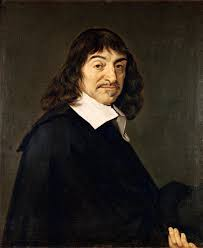
\includegraphics[width=0.8\linewidth]{dikaer.jpg}
				
				% If you want a caption for your figure, you can use the figure environment:
				% \begin{figure}
					%     \includegraphics[width=\linewidth]{your_figure_filename.png}
					%     \caption{This is a caption for the figure.}
					% \end{figure}
			\end{column}
			
			% Right Column for the Text
			\begin{column}{0.50\textwidth} % Adjust width as needed (e.g., 0.45\textwidth)
				This is where your descriptive text will go.
				You can use standard LaTeX formatting here.
				\begin{itemize}
					\item Explain key aspects of the figure.
					\item Provide supporting details.
					\item Or list important takeaways.
				\end{itemize}
				More text can follow here, describing the content further.
			\end{column}
			
		\end{columns}
	\end{frame}
	
\end{document}
